% Options for packages loaded elsewhere
\PassOptionsToPackage{unicode}{hyperref}
\PassOptionsToPackage{hyphens}{url}
%
\documentclass[
]{article}
\usepackage{amsmath,amssymb}
\usepackage{iftex}
\ifPDFTeX
  \usepackage[T1]{fontenc}
  \usepackage[utf8]{inputenc}
  \usepackage{textcomp} % provide euro and other symbols
\else % if luatex or xetex
  \usepackage{unicode-math} % this also loads fontspec
  \defaultfontfeatures{Scale=MatchLowercase}
  \defaultfontfeatures[\rmfamily]{Ligatures=TeX,Scale=1}
\fi
\usepackage{lmodern}
\ifPDFTeX\else
  % xetex/luatex font selection
\fi
% Use upquote if available, for straight quotes in verbatim environments
\IfFileExists{upquote.sty}{\usepackage{upquote}}{}
\IfFileExists{microtype.sty}{% use microtype if available
  \usepackage[]{microtype}
  \UseMicrotypeSet[protrusion]{basicmath} % disable protrusion for tt fonts
}{}
\makeatletter
\@ifundefined{KOMAClassName}{% if non-KOMA class
  \IfFileExists{parskip.sty}{%
    \usepackage{parskip}
  }{% else
    \setlength{\parindent}{0pt}
    \setlength{\parskip}{6pt plus 2pt minus 1pt}}
}{% if KOMA class
  \KOMAoptions{parskip=half}}
\makeatother
\usepackage{xcolor}
\usepackage[margin=1in]{geometry}
\usepackage{color}
\usepackage{fancyvrb}
\newcommand{\VerbBar}{|}
\newcommand{\VERB}{\Verb[commandchars=\\\{\}]}
\DefineVerbatimEnvironment{Highlighting}{Verbatim}{commandchars=\\\{\}}
% Add ',fontsize=\small' for more characters per line
\usepackage{framed}
\definecolor{shadecolor}{RGB}{248,248,248}
\newenvironment{Shaded}{\begin{snugshade}}{\end{snugshade}}
\newcommand{\AlertTok}[1]{\textcolor[rgb]{0.94,0.16,0.16}{#1}}
\newcommand{\AnnotationTok}[1]{\textcolor[rgb]{0.56,0.35,0.01}{\textbf{\textit{#1}}}}
\newcommand{\AttributeTok}[1]{\textcolor[rgb]{0.13,0.29,0.53}{#1}}
\newcommand{\BaseNTok}[1]{\textcolor[rgb]{0.00,0.00,0.81}{#1}}
\newcommand{\BuiltInTok}[1]{#1}
\newcommand{\CharTok}[1]{\textcolor[rgb]{0.31,0.60,0.02}{#1}}
\newcommand{\CommentTok}[1]{\textcolor[rgb]{0.56,0.35,0.01}{\textit{#1}}}
\newcommand{\CommentVarTok}[1]{\textcolor[rgb]{0.56,0.35,0.01}{\textbf{\textit{#1}}}}
\newcommand{\ConstantTok}[1]{\textcolor[rgb]{0.56,0.35,0.01}{#1}}
\newcommand{\ControlFlowTok}[1]{\textcolor[rgb]{0.13,0.29,0.53}{\textbf{#1}}}
\newcommand{\DataTypeTok}[1]{\textcolor[rgb]{0.13,0.29,0.53}{#1}}
\newcommand{\DecValTok}[1]{\textcolor[rgb]{0.00,0.00,0.81}{#1}}
\newcommand{\DocumentationTok}[1]{\textcolor[rgb]{0.56,0.35,0.01}{\textbf{\textit{#1}}}}
\newcommand{\ErrorTok}[1]{\textcolor[rgb]{0.64,0.00,0.00}{\textbf{#1}}}
\newcommand{\ExtensionTok}[1]{#1}
\newcommand{\FloatTok}[1]{\textcolor[rgb]{0.00,0.00,0.81}{#1}}
\newcommand{\FunctionTok}[1]{\textcolor[rgb]{0.13,0.29,0.53}{\textbf{#1}}}
\newcommand{\ImportTok}[1]{#1}
\newcommand{\InformationTok}[1]{\textcolor[rgb]{0.56,0.35,0.01}{\textbf{\textit{#1}}}}
\newcommand{\KeywordTok}[1]{\textcolor[rgb]{0.13,0.29,0.53}{\textbf{#1}}}
\newcommand{\NormalTok}[1]{#1}
\newcommand{\OperatorTok}[1]{\textcolor[rgb]{0.81,0.36,0.00}{\textbf{#1}}}
\newcommand{\OtherTok}[1]{\textcolor[rgb]{0.56,0.35,0.01}{#1}}
\newcommand{\PreprocessorTok}[1]{\textcolor[rgb]{0.56,0.35,0.01}{\textit{#1}}}
\newcommand{\RegionMarkerTok}[1]{#1}
\newcommand{\SpecialCharTok}[1]{\textcolor[rgb]{0.81,0.36,0.00}{\textbf{#1}}}
\newcommand{\SpecialStringTok}[1]{\textcolor[rgb]{0.31,0.60,0.02}{#1}}
\newcommand{\StringTok}[1]{\textcolor[rgb]{0.31,0.60,0.02}{#1}}
\newcommand{\VariableTok}[1]{\textcolor[rgb]{0.00,0.00,0.00}{#1}}
\newcommand{\VerbatimStringTok}[1]{\textcolor[rgb]{0.31,0.60,0.02}{#1}}
\newcommand{\WarningTok}[1]{\textcolor[rgb]{0.56,0.35,0.01}{\textbf{\textit{#1}}}}
\usepackage{graphicx}
\makeatletter
\def\maxwidth{\ifdim\Gin@nat@width>\linewidth\linewidth\else\Gin@nat@width\fi}
\def\maxheight{\ifdim\Gin@nat@height>\textheight\textheight\else\Gin@nat@height\fi}
\makeatother
% Scale images if necessary, so that they will not overflow the page
% margins by default, and it is still possible to overwrite the defaults
% using explicit options in \includegraphics[width, height, ...]{}
\setkeys{Gin}{width=\maxwidth,height=\maxheight,keepaspectratio}
% Set default figure placement to htbp
\makeatletter
\def\fps@figure{htbp}
\makeatother
\setlength{\emergencystretch}{3em} % prevent overfull lines
\providecommand{\tightlist}{%
  \setlength{\itemsep}{0pt}\setlength{\parskip}{0pt}}
\setcounter{secnumdepth}{5}
\ifLuaTeX
  \usepackage{selnolig}  % disable illegal ligatures
\fi
\usepackage{bookmark}
\IfFileExists{xurl.sty}{\usepackage{xurl}}{} % add URL line breaks if available
\urlstyle{same}
\hypersetup{
  pdftitle={Bellabeat\_Capstone\_Project},
  pdfauthor={Baraka Mtana},
  hidelinks,
  pdfcreator={LaTeX via pandoc}}

\title{Bellabeat\_Capstone\_Project}
\author{Baraka Mtana}
\date{2024-10-16}

\begin{document}
\maketitle

\begin{Shaded}
\begin{Highlighting}[]
\CommentTok{\# Set up environment}
\CommentTok{\# import libraries}
\FunctionTok{library}\NormalTok{(tidyverse)}
\end{Highlighting}
\end{Shaded}

\begin{verbatim}
## -- Attaching core tidyverse packages ------------------------ tidyverse 2.0.0 --
## v dplyr     1.1.4     v readr     2.1.5
## v forcats   1.0.0     v stringr   1.5.1
## v ggplot2   3.5.1     v tibble    3.2.1
## v lubridate 1.9.3     v tidyr     1.3.1
## v purrr     1.0.2     
## -- Conflicts ------------------------------------------ tidyverse_conflicts() --
## x dplyr::filter() masks stats::filter()
## x dplyr::lag()    masks stats::lag()
## i Use the conflicted package (<http://conflicted.r-lib.org/>) to force all conflicts to become errors
\end{verbatim}

\begin{Shaded}
\begin{Highlighting}[]
\CommentTok{\# install.packages("lubridate")}
\FunctionTok{library}\NormalTok{(lubridate)}
\FunctionTok{library}\NormalTok{(ggplot2)}
\FunctionTok{library}\NormalTok{(dplyr)}
\end{Highlighting}
\end{Shaded}

\begin{Shaded}
\begin{Highlighting}[]
\CommentTok{\# get and print working directory}
\NormalTok{currentDir }\OtherTok{\textless{}{-}} \FunctionTok{getwd}\NormalTok{() }
\FunctionTok{print}\NormalTok{(currentDir)}
\end{Highlighting}
\end{Shaded}

\begin{verbatim}
## [1] "C:/Users/LENOVO/Desktop/Bellabeat_Capstone-project"
\end{verbatim}

\begin{Shaded}
\begin{Highlighting}[]
\CommentTok{\# list file in the working DIR}
\FunctionTok{list.files}\NormalTok{(currentDir)}
\end{Highlighting}
\end{Shaded}

\begin{verbatim}
##  [1] "Bellabeat_Capstone-project.R"                                                                                                  
##  [2] "Bellabeat_Capstone-project.Rproj"                                                                                              
##  [3] "Bellabeat_Capstone_Project.html"                                                                                               
##  [4] "Bellabeat_Capstone_Project.log"                                                                                                
##  [5] "Bellabeat_Capstone_Project.tex"                                                                                                
##  [6] "BellabeatCapstoneProject.log"                                                                                                  
##  [7] "BellabeatCapstoneProject.Rmd"                                                                                                  
##  [8] "BellabeatCapstoneProject.tex"                                                                                                  
##  [9] "BellabeatCapstoneProject_files"                                                                                                
## [10] "customer_averages.csv"                                                                                                         
## [11] "LICENSE"                                                                                                                       
## [12] "mturkfitbit_export_3.12.16-4.11.16"                                                                                            
## [13] "README.md"                                                                                                                     
## [14] "Screenshot.png"                                                                                                                
## [15] "UYTzmqN3SS-WCbei0buGkw_cbefaed7e1354ffb8e992c8e198906f1_Case-Study-2_-How-can-a-wellness-technology-company-play-it-smart-.pdf"
\end{verbatim}

\begin{Shaded}
\begin{Highlighting}[]
\CommentTok{\# we are interested in the csv files in \textquotesingle{}mturkfitbit\_export\_3.12.16{-}4.11.16\textquotesingle{}}
\CommentTok{\# and \textquotesingle{}Fitabase Data 3.12.16{-}4.11.16\textquotesingle{}}
\NormalTok{csv\_files\_Dir }\OtherTok{\textless{}{-}} \FunctionTok{file.path}\NormalTok{(}
\NormalTok{  currentDir, }\StringTok{\textquotesingle{}mturkfitbit\_export\_3.12.16{-}4.11.16\textquotesingle{}}\NormalTok{, }\StringTok{\textquotesingle{}Fitabase Data 3.12.16{-}4.11.16\textquotesingle{}}
\NormalTok{)}

\NormalTok{csv\_files }\OtherTok{\textless{}{-}} \FunctionTok{list.files}\NormalTok{(csv\_files\_Dir)}
\NormalTok{len\_cvs }\OtherTok{=} \FunctionTok{length}\NormalTok{(csv\_files)}

\CommentTok{\# csv\_files \textless{}{-} list.files(csv\_files\_Dir, pattern = "\textbackslash{}\textbackslash{}.csv$", full.names = TRUE)}
\CommentTok{\# print(csv\_files)}
\end{Highlighting}
\end{Shaded}

\begin{Shaded}
\begin{Highlighting}[]
\CommentTok{\# Initialize an empty list to store data frames}
\NormalTok{dfs }\OtherTok{\textless{}{-}} \FunctionTok{list}\NormalTok{()}


\ControlFlowTok{for}\NormalTok{ (file }\ControlFlowTok{in}\NormalTok{ csv\_files) \{}
  
  \FunctionTok{print}\NormalTok{(}\FunctionTok{paste}\NormalTok{(}\StringTok{"Working on"}\NormalTok{, file))}
  
  \CommentTok{\# create df names}
  \CommentTok{\# split the file name str character}
\NormalTok{  df\_name }\OtherTok{\textless{}{-}} \FunctionTok{strsplit}\NormalTok{(file, }\AttributeTok{split =} \StringTok{\textquotesingle{}}\SpecialCharTok{\textbackslash{}\textbackslash{}}\StringTok{.\textquotesingle{}}\NormalTok{)[[}\DecValTok{1}\NormalTok{]] }\CommentTok{\#Access the first and only string}
  
  \CommentTok{\# get the first part of the string character which is basically the name }
  \CommentTok{\# without the csv extension}
\NormalTok{  df\_name }\OtherTok{\textless{}{-}}\NormalTok{ df\_name[}\DecValTok{1}\NormalTok{]}
  
  \CommentTok{\# concatenate the df\_name with df}
\NormalTok{  df\_name }\OtherTok{\textless{}{-}} \FunctionTok{paste0}\NormalTok{(df\_name, }\StringTok{"\_df"}\NormalTok{) }\CommentTok{\# Use paste0 for no space between parts}
  
  \CommentTok{\# create full path for each file so that we can import them}
\NormalTok{  filepath }\OtherTok{\textless{}{-}} \FunctionTok{file.path}\NormalTok{(csv\_files\_Dir, file)}
  
  \CommentTok{\# read csv }
\NormalTok{  df }\OtherTok{\textless{}{-}} \FunctionTok{read.csv}\NormalTok{((filepath))}
  
  \CommentTok{\# append dfs and their names}
\NormalTok{  dfs[[df\_name]] }\OtherTok{\textless{}{-}}\NormalTok{ df  }\CommentTok{\# Store the data frame in the list, keyed by file path}

\NormalTok{\}}
\end{Highlighting}
\end{Shaded}

\begin{verbatim}
## [1] "Working on dailyActivity_merged.csv"
## [1] "Working on heartrate_seconds_merged.csv"
## [1] "Working on hourlyCalories_merged.csv"
## [1] "Working on hourlyIntensities_merged.csv"
## [1] "Working on hourlySteps_merged.csv"
## [1] "Working on minuteCaloriesNarrow_merged.csv"
## [1] "Working on minuteIntensitiesNarrow_merged.csv"
## [1] "Working on minuteMETsNarrow_merged.csv"
## [1] "Working on minuteSleep_merged.csv"
## [1] "Working on minuteStepsNarrow_merged.csv"
## [1] "Working on weightLogInfo_merged.csv"
\end{verbatim}

\begin{Shaded}
\begin{Highlighting}[]
\CommentTok{\# Confirm that all df were read successfully}
\ControlFlowTok{if}\NormalTok{ (len\_cvs }\SpecialCharTok{==} \FunctionTok{length}\NormalTok{(dfs)) \{}
  \FunctionTok{print}\NormalTok{(}\StringTok{"All files read successfully"}\NormalTok{)}
\NormalTok{\} }\ControlFlowTok{else}\NormalTok{ \{}
  \FunctionTok{print}\NormalTok{(}\StringTok{"Some files were not read correctly"}\NormalTok{)}
\NormalTok{\}}
\end{Highlighting}
\end{Shaded}

\begin{verbatim}
## [1] "All files read successfully"
\end{verbatim}

\begin{Shaded}
\begin{Highlighting}[]
\FunctionTok{print}\NormalTok{(}\FunctionTok{names}\NormalTok{(dfs))}
\end{Highlighting}
\end{Shaded}

\begin{verbatim}
##  [1] "dailyActivity_merged_df"           "heartrate_seconds_merged_df"      
##  [3] "hourlyCalories_merged_df"          "hourlyIntensities_merged_df"      
##  [5] "hourlySteps_merged_df"             "minuteCaloriesNarrow_merged_df"   
##  [7] "minuteIntensitiesNarrow_merged_df" "minuteMETsNarrow_merged_df"       
##  [9] "minuteSleep_merged_df"             "minuteStepsNarrow_merged_df"      
## [11] "weightLogInfo_merged_df"
\end{verbatim}

\begin{Shaded}
\begin{Highlighting}[]
\CommentTok{\# Here we\textquotesingle{}ll write function we\textquotesingle{}ll reuse}

\CommentTok{\# Check for missing values}
\NormalTok{missing\_value }\OtherTok{\textless{}{-}} \ControlFlowTok{function}\NormalTok{(df)\{}
  \FunctionTok{print}\NormalTok{(}\FunctionTok{paste}\NormalTok{(}\StringTok{"Count of total missing values"}\NormalTok{, }\FunctionTok{sum}\NormalTok{(}\FunctionTok{is.na}\NormalTok{(df))))}
\NormalTok{\}}


\CommentTok{\# get number of unique values}
\NormalTok{unique\_value }\OtherTok{\textless{}{-}} \ControlFlowTok{function}\NormalTok{(df, column\_of\_interest) \{}
  \CommentTok{\#get the unique values}
\NormalTok{  uniques }\OtherTok{\textless{}{-}} \FunctionTok{unique}\NormalTok{(df[[column\_of\_interest]])}
  
  \CommentTok{\# Get the unique values from the specified column}
\NormalTok{  n\_unique }\OtherTok{\textless{}{-}} \FunctionTok{length}\NormalTok{(uniques)}
  
  \FunctionTok{print}\NormalTok{(}\FunctionTok{paste}\NormalTok{(column\_of\_interest, }\StringTok{"has"}\NormalTok{,  n\_unique, }\StringTok{"values"}\NormalTok{))}
  
\NormalTok{\}}



\NormalTok{N\_unique\_char }\OtherTok{\textless{}{-}} \ControlFlowTok{function}\NormalTok{(df, column\_of\_interest)\{}
  \CommentTok{\# Initialize/ pre{-}allocate a numeric vector of a specific length, initialized with   zeros}
\NormalTok{  n\_char }\OtherTok{\textless{}{-}} \FunctionTok{numeric}\NormalTok{(}\FunctionTok{nrow}\NormalTok{(df)) }
  
  \ControlFlowTok{for}\NormalTok{ (i }\ControlFlowTok{in} \FunctionTok{seq\_along}\NormalTok{(df[[column\_of\_interest]]))\{}
\NormalTok{    n\_char[i] }\OtherTok{\textless{}{-}} \FunctionTok{nchar}\NormalTok{(df[[column\_of\_interest]][i])}
\NormalTok{  \}}
  
  \CommentTok{\# get the number of unique characters}
\NormalTok{  character\_lens }\OtherTok{\textless{}{-}} \FunctionTok{unique}\NormalTok{(n\_char)}
  
  \FunctionTok{return}\NormalTok{(character\_lens)}
\NormalTok{\}}
  

\CommentTok{\# change column to datetime}
\NormalTok{change\_to\_date }\OtherTok{\textless{}{-}} \ControlFlowTok{function}\NormalTok{(df, column\_of\_interest)\{}
\NormalTok{  df[[column\_of\_interest]] }\OtherTok{\textless{}{-}} 
      \FunctionTok{as.POSIXct}\NormalTok{(}
\NormalTok{      df[[column\_of\_interest]],}
      \AttributeTok{format=}\StringTok{"\%m/\%d/\%Y"}\NormalTok{ ,}\AttributeTok{tz=}\FunctionTok{Sys.timezone}\NormalTok{()}
\NormalTok{      )}
  \CommentTok{\# confirm the datatype of the column of interest}
  \FunctionTok{print}\NormalTok{(}\FunctionTok{paste}\NormalTok{(column\_of\_interest, }\StringTok{"has"}\NormalTok{ ,}\FunctionTok{class}\NormalTok{(df[[column\_of\_interest]]) , }\StringTok{"datatype"}\NormalTok{))}
  
  \FunctionTok{print}\NormalTok{(}\FunctionTok{head}\NormalTok{(df[column\_of\_interest], }\DecValTok{10}\NormalTok{))}
  
  
  \FunctionTok{return}\NormalTok{(df)}
  
\NormalTok{\}}

\CommentTok{\# Check if the columns are identical}
\NormalTok{identical\_columns }\OtherTok{\textless{}{-}} \ControlFlowTok{function}\NormalTok{(df, col1, col2)\{}
  \ControlFlowTok{if}\NormalTok{ (}\FunctionTok{identical}\NormalTok{(df[[col1]], df[[col2]])) \{}
    \FunctionTok{print}\NormalTok{(}\StringTok{"The columns are identical."}\NormalTok{)}
\NormalTok{  \} }\ControlFlowTok{else}\NormalTok{ \{}
    \FunctionTok{print}\NormalTok{(}\StringTok{"The columns are NOT identical."}\NormalTok{)}
\NormalTok{  \} }
\NormalTok{\}}


\CommentTok{\# calculate averages}
\NormalTok{averages }\OtherTok{\textless{}{-}} \ControlFlowTok{function}\NormalTok{(df)\{}
\NormalTok{  averages\_per\_athlete }\OtherTok{\textless{}{-}}\NormalTok{ df }\SpecialCharTok{\%\textgreater{}\%}
    \FunctionTok{group\_by}\NormalTok{(Id)  }\SpecialCharTok{\%\textgreater{}\%}
      \FunctionTok{summarise}\NormalTok{(}
        \AttributeTok{Avg\_Steps =} \FunctionTok{mean}\NormalTok{(TotalSteps),}
        \AttributeTok{Avg\_Distance =} \FunctionTok{mean}\NormalTok{(TotalDistance),}
        \AttributeTok{Avg\_TrackedDistance =} \FunctionTok{mean}\NormalTok{(TrackerDistance),}
        \AttributeTok{Avg\_LoggedActivityDistance =} \FunctionTok{mean}\NormalTok{(LoggedActivitiesDistance),}
        \AttributeTok{Avg\_VeryActiveDistance =} \FunctionTok{mean}\NormalTok{(VeryActiveDistance),}
        \AttributeTok{Avg\_ModeratelyActiveDistance =} \FunctionTok{mean}\NormalTok{(ModeratelyActiveDistance),}
        \AttributeTok{Avg\_LightActiveDistance =} \FunctionTok{mean}\NormalTok{(LightActiveDistance),}
        \AttributeTok{Avg\_SedentaryActiveDistance =} \FunctionTok{mean}\NormalTok{(SedentaryActiveDistance),}
        \AttributeTok{Avg\_Calories =} \FunctionTok{mean}\NormalTok{(Calories)}
\NormalTok{    )}
  
  \FunctionTok{write.csv}\NormalTok{(averages\_per\_athlete, }\StringTok{"customer\_averages.csv"}\NormalTok{, }\AttributeTok{row.names =} \ConstantTok{FALSE}\NormalTok{)}
  
  \FunctionTok{print}\NormalTok{(}\FunctionTok{head}\NormalTok{(averages\_per\_athlete, }\DecValTok{5}\NormalTok{))}
\NormalTok{\}}


\CommentTok{\# line plot function }
\NormalTok{line\_plot }\OtherTok{\textless{}{-}} \ControlFlowTok{function}\NormalTok{(df, x\_col, y\_col)\{}
  \FunctionTok{ggplot}\NormalTok{ (}\AttributeTok{data =}\NormalTok{ df) }\SpecialCharTok{+}
    \FunctionTok{geom\_line}\NormalTok{(}\AttributeTok{mapping =} \FunctionTok{aes}\NormalTok{(}\AttributeTok{x=}\NormalTok{ .data[[x\_col]] , }\AttributeTok{y=}\NormalTok{ .data[[y\_col]] )) }\SpecialCharTok{+}
    \FunctionTok{labs}\NormalTok{(}\AttributeTok{title =} \FunctionTok{paste}\NormalTok{(x\_col, }\StringTok{"and"}\NormalTok{, y\_col, }\StringTok{"relationsip"}\NormalTok{))}
\NormalTok{\}}
\end{Highlighting}
\end{Shaded}

\begin{Shaded}
\begin{Highlighting}[]
\NormalTok{dailyActivity\_merged\_df }\OtherTok{\textless{}{-}}\NormalTok{dfs[[}\StringTok{"dailyActivity\_merged\_df"}\NormalTok{]]}
\FunctionTok{str}\NormalTok{(dailyActivity\_merged\_df)}
\end{Highlighting}
\end{Shaded}

\begin{verbatim}
## 'data.frame':    457 obs. of  15 variables:
##  $ Id                      : num  1.5e+09 1.5e+09 1.5e+09 1.5e+09 1.5e+09 ...
##  $ ActivityDate            : chr  "3/25/2016" "3/26/2016" "3/27/2016" "3/28/2016" ...
##  $ TotalSteps              : int  11004 17609 12736 13231 12041 10970 12256 12262 11248 10016 ...
##  $ TotalDistance           : num  7.11 11.55 8.53 8.93 7.85 ...
##  $ TrackerDistance         : num  7.11 11.55 8.53 8.93 7.85 ...
##  $ LoggedActivitiesDistance: num  0 0 0 0 0 0 0 0 0 0 ...
##  $ VeryActiveDistance      : num  2.57 6.92 4.66 3.19 2.16 ...
##  $ ModeratelyActiveDistance: num  0.46 0.73 0.16 0.79 1.09 ...
##  $ LightActiveDistance     : num  4.07 3.91 3.71 4.95 4.61 ...
##  $ SedentaryActiveDistance : num  0 0 0 0 0 0 0 0 0 0 ...
##  $ VeryActiveMinutes       : int  33 89 56 39 28 30 33 47 40 15 ...
##  $ FairlyActiveMinutes     : int  12 17 5 20 28 13 12 21 11 30 ...
##  $ LightlyActiveMinutes    : int  205 274 268 224 243 223 239 200 244 314 ...
##  $ SedentaryMinutes        : int  804 588 605 1080 763 1174 820 866 636 655 ...
##  $ Calories                : int  1819 2154 1944 1932 1886 1820 1889 1868 1843 1850 ...
\end{verbatim}

\begin{Shaded}
\begin{Highlighting}[]
\CommentTok{\# we\textquotesingle{}ll have a look at all unique value in if non of them is repeated}
\CommentTok{\# change ActivityDate from character to datetime}
\CommentTok{\# Assuming TotalSteps is cadence we\textquotesingle{}ll see the average length of a step per person}
\CommentTok{\# See if TotalDistance and TrackerDistance distance record the same data}
\CommentTok{\# Calculate average TotalDistance, TrackerDistance, VeryActiveDistance, }
\CommentTok{\# ModeratelyActiveDistance, LightActiveDistance, SedentaryActiveDistance,}
\CommentTok{\# Average calories lost per day}
\end{Highlighting}
\end{Shaded}

Check for missing values in dailyActivity\_merged\_df

\begin{Shaded}
\begin{Highlighting}[]
\FunctionTok{missing\_value}\NormalTok{(dailyActivity\_merged\_df)}
\end{Highlighting}
\end{Shaded}

\begin{verbatim}
## [1] "Count of total missing values 0"
\end{verbatim}

check how many customers are we dealing with

\begin{Shaded}
\begin{Highlighting}[]
\CommentTok{\# call function on dailyActivity\_merged\_df}
\FunctionTok{unique\_value}\NormalTok{(dailyActivity\_merged\_df, }\StringTok{"Id"}\NormalTok{)}
\end{Highlighting}
\end{Shaded}

\begin{verbatim}
## [1] "Id has 35 values"
\end{verbatim}

\section{see the number of character in each character of the
ActivityDate
column}\label{see-the-number-of-character-in-each-character-of-the-activitydate-column}

\section{since we've already seen there are inconsistencies in the
ActivityDate,
--\textgreater{}}\label{since-weve-already-seen-there-are-inconsistencies-in-the-activitydate}

\section{let's see if there are some date characters saved with
hrs,min,and
secs}\label{lets-see-if-there-are-some-date-characters-saved-with-hrsminand-secs}

\begin{Shaded}
\begin{Highlighting}[]
\CommentTok{\# see if there is uniformity in the Activity date columns}
\FunctionTok{N\_unique\_char}\NormalTok{(dailyActivity\_merged\_df, }\StringTok{"ActivityDate"}\NormalTok{)}
\end{Highlighting}
\end{Shaded}

\begin{verbatim}
## [1] 9 8
\end{verbatim}

We have different datatypes let's see if this will affect how changing
the datatype of ActivityDate

\begin{Shaded}
\begin{Highlighting}[]
\CommentTok{\# see if there is uniformity in the Activity date columns}
\FunctionTok{N\_unique\_char}\NormalTok{(dailyActivity\_merged\_df, }\StringTok{"ActivityDate"}\NormalTok{)}
\end{Highlighting}
\end{Shaded}

\begin{verbatim}
## [1] 9 8
\end{verbatim}

\begin{Shaded}
\begin{Highlighting}[]
\CommentTok{\# call change\_to\_date on dailyActivity\_merged\_df}
\NormalTok{dailyActivity\_merged\_df }\OtherTok{\textless{}{-}} \FunctionTok{change\_to\_date}\NormalTok{(dailyActivity\_merged\_df, }\StringTok{"ActivityDate"}\NormalTok{)}
\end{Highlighting}
\end{Shaded}

\begin{verbatim}
## [1] "ActivityDate has POSIXct datatype" "ActivityDate has POSIXt datatype" 
##    ActivityDate
## 1    2016-03-25
## 2    2016-03-26
## 3    2016-03-27
## 4    2016-03-28
## 5    2016-03-29
## 6    2016-03-30
## 7    2016-03-31
## 8    2016-04-01
## 9    2016-04-02
## 10   2016-04-03
\end{verbatim}

\begin{Shaded}
\begin{Highlighting}[]
\CommentTok{\# call identical\_columns on dailyActivity\_merged\_df}
\FunctionTok{identical\_columns}\NormalTok{(dailyActivity\_merged\_df, }\StringTok{"TotalDistance"}\NormalTok{, }\StringTok{"TrackerDistance"}\NormalTok{ )}
\end{Highlighting}
\end{Shaded}

\begin{verbatim}
## [1] "The columns are NOT identical."
\end{verbatim}

\begin{Shaded}
\begin{Highlighting}[]
\FunctionTok{averages}\NormalTok{(dailyActivity\_merged\_df)}
\end{Highlighting}
\end{Shaded}

\begin{verbatim}
## # A tibble: 5 x 10
##           Id Avg_Steps Avg_Distance Avg_TrackedDistance Avg_LoggedActivityDist~1
##        <dbl>     <dbl>        <dbl>               <dbl>                    <dbl>
## 1 1503960366    11641.         7.61                7.61                        0
## 2 1624580081     4226.         2.75                2.75                        0
## 3 1644430081     9275.         6.75                6.75                        0
## 4 1844505072     3641.         2.41                2.41                        0
## 5 1927972279     2181.         1.51                1.51                        0
## # i abbreviated name: 1: Avg_LoggedActivityDistance
## # i 5 more variables: Avg_VeryActiveDistance <dbl>,
## #   Avg_ModeratelyActiveDistance <dbl>, Avg_LightActiveDistance <dbl>,
## #   Avg_SedentaryActiveDistance <dbl>, Avg_Calories <dbl>
\end{verbatim}

\begin{Shaded}
\begin{Highlighting}[]
\CommentTok{\# call function on dailyActivity\_merged\_df }
\FunctionTok{line\_plot}\NormalTok{(}\AttributeTok{df =}\NormalTok{ dailyActivity\_merged\_df, }\AttributeTok{x\_col=} \StringTok{"Calories"}\NormalTok{, }\AttributeTok{y\_col =} \StringTok{"TotalDistance"}\NormalTok{)}
\end{Highlighting}
\end{Shaded}

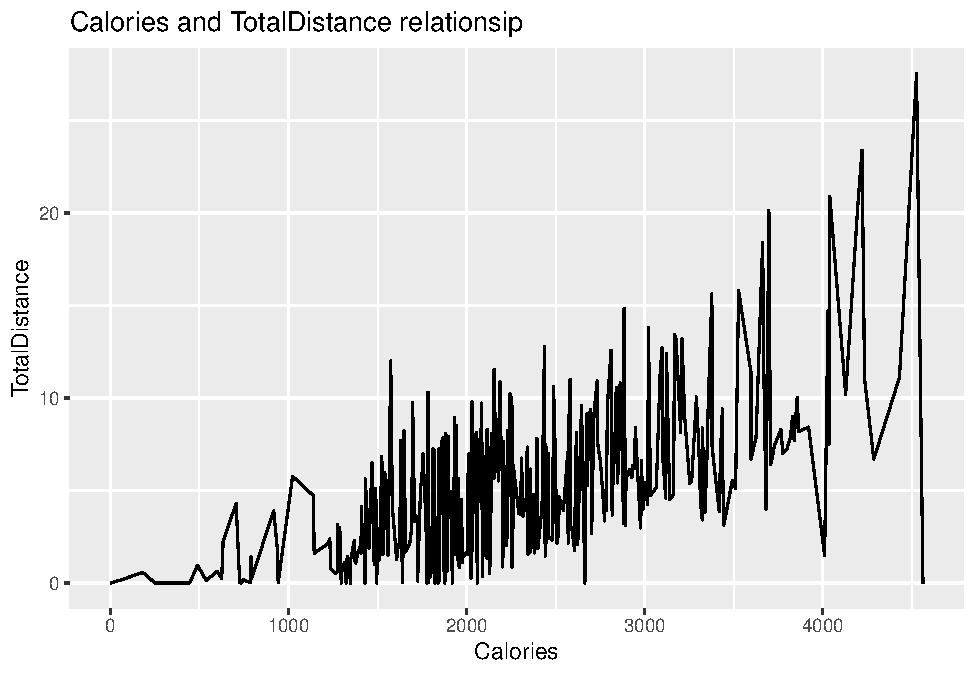
\includegraphics{BellabeatCapstoneProject_files/figure-latex/unnamed-chunk-15-1.pdf}
There is a positive correlation between Calories and TotalDistance the
is

\subsection{Let's get to see
heartrate\_seconds\_merged\_df}\label{lets-get-to-see-heartrate_seconds_merged_df}

\begin{Shaded}
\begin{Highlighting}[]
\NormalTok{heartrate\_seconds\_merged\_df }\OtherTok{\textless{}{-}}\NormalTok{ dfs[[}\StringTok{"heartrate\_seconds\_merged\_df"}\NormalTok{]]}
\FunctionTok{str}\NormalTok{(heartrate\_seconds\_merged\_df)}
\end{Highlighting}
\end{Shaded}

\begin{verbatim}
## 'data.frame':    1154681 obs. of  3 variables:
##  $ Id   : num  2.02e+09 2.02e+09 2.02e+09 2.02e+09 2.02e+09 ...
##  $ Time : chr  "4/1/2016 7:54:00 AM" "4/1/2016 7:54:05 AM" "4/1/2016 7:54:10 AM" "4/1/2016 7:54:15 AM" ...
##  $ Value: int  93 91 96 98 100 101 104 105 102 106 ...
\end{verbatim}

\begin{Shaded}
\begin{Highlighting}[]
\CommentTok{\# Check if the unique Ids are similar to the ones in dailyActivity\_merged\_df}
\CommentTok{\# change time column to datetime}
\CommentTok{\# see the average heart rate per unique id, see the correlation between the average heart rate and calories lost}
\CommentTok{\# see if there is any negative hr values}
\end{Highlighting}
\end{Shaded}

\begin{Shaded}
\begin{Highlighting}[]
\CommentTok{\#Check for missing values in heartrate\_seconds\_merged\_df}
\FunctionTok{missing\_value}\NormalTok{(heartrate\_seconds\_merged\_df)}
\end{Highlighting}
\end{Shaded}

\begin{verbatim}
## [1] "Count of total missing values 0"
\end{verbatim}

\end{document}
